\documentclass{article}
\usepackage[utf8]{inputenc}
\usepackage{graphicx}
\usepackage{float}
\usepackage[dvipsnames]{xcolor}
\usepackage[left=1in,top=1in,right=1in,bottom=1in]{geometry}

\title{notes\_for\_three\_easy\_pieces}

\begin{document}


\maketitle
\tableofcontents
\pagebreak

\section{Virtualization}
\subsection{Processes}
\subsubsection{Definition}
A running program. The program
itself is a lifeless thing: it just sits there on the disk, a bunch of instructions
(and maybe some static data), waiting to spring into action.

\subsubsection{How To Provide The Illusion of Many CPUs}
The OS creates this illusion by \textbf{\color{red}virtualizing} the CPU. By running one
process, then stopping it and running another, and so forth, the OS can
promote the illusion that many virtual CPUs exist when in fact there is
only one physical CPU (or a few).\textbf{\color{red}Time
sharing of the CPU}, allows users to run as many concurrent processes as
they would like; \textbf{\color{red}the potential cost is performance,} as each will run more
slowly if the CPU(s) must be shared.
\subsubsection{Implement Virtualization of CPU}
\begin{itemize}
    \item \textbf{mechanisms: }low-level methods or protocols that implement a needed piece of functionality.
    \item \textbf{policies: }Policies are algorithms for making some kind of decision within the OS, e.g. \textbf{scheduling policy}
\end{itemize}

\subsubsection{Time Sharing \& Space Sharing}
\begin{itemize}
    \item \textbf{Time sharing} is a basic technique used by an OS to share a resource. By allowing the resource to be used for a little while by one entity, and then a little while by another, and so forth, the resource in question (e.g., the CPU, or a network link) can be shared by many.
    \item \textbf{Space sharing} where a resource is divided (in space) among those who wish to use it.
\end{itemize}

\subsubsection{Machine State}
To understand what constitutes a process, we thus have to understand
its machine state
\begin{itemize}
    \item \textbf{memory (address space): }What's in memory: instructions, data
    
    \item \textbf{registers: }many instructions
explicitly read or update registers. Some particularly special registers like
    \begin{itemize}
        \item \textbf{program counter (PC) or called instruction pointer(IP): }which instruction of the program
    will execute next
    \item \textbf{stack pointer and asscoiated frame pointer: }manage the stack for function parameters, local variables,
    and return addresses.
    \end{itemize}
    
    \item \textbf{I/O information: }include a list of the files the process currently has open

\end{itemize}

\subsubsection{Process API}
\begin{itemize}
    \item \textbf{Create: }
    \item \textbf{Destory: }
    \item \textbf{Wait: }
    \item \textbf{Miscellaneous Control: }most operating systems provide some kind of method to suspend a process (stop it from running for a while) and then resume it (continue it running).
    \item \textbf{Status: }
\end{itemize}


\subsubsection{process creation}
How does the OS get a program up
and running? How does process creation actually work?
\begin{itemize}
    \item \textbf{Load:} load code and any static data (e.g., initialized variables) into memory, into the address space of the process. Programs initially reside on \textbf{disk or flash-based SSDs} in some kind of executable format;
    
    \item \textbf{when loading happens: }In early (or simple) operating systems, the loading process is done all at once before running the program; modern OSes perform the process lazily, i.e., by loading pieces of code or data only as they are needed during program execution
    
    \item \textbf{allcate some memory for program's run-time stack} C uses stack for \textbf{local variables, function parameters and return addresses}
    
    \item \textbf{allocate some memory for the program’s heap: } C uses heap for explicitly requested dynamically-allocated data; programs request such space by calling malloc() and free it explicitly by calling free().e.g. data structures like \textbf{linked list, hash tables, trees and so on}. The heap will grow larger
    
    \item \textbf{initialization tasks like input/output (I/O)}in UNIX systems, each process by default has three open \textbf{file descriptors}, for standard input, output, and error;
\end{itemize}

\begin{figure}[H]
    \centering
    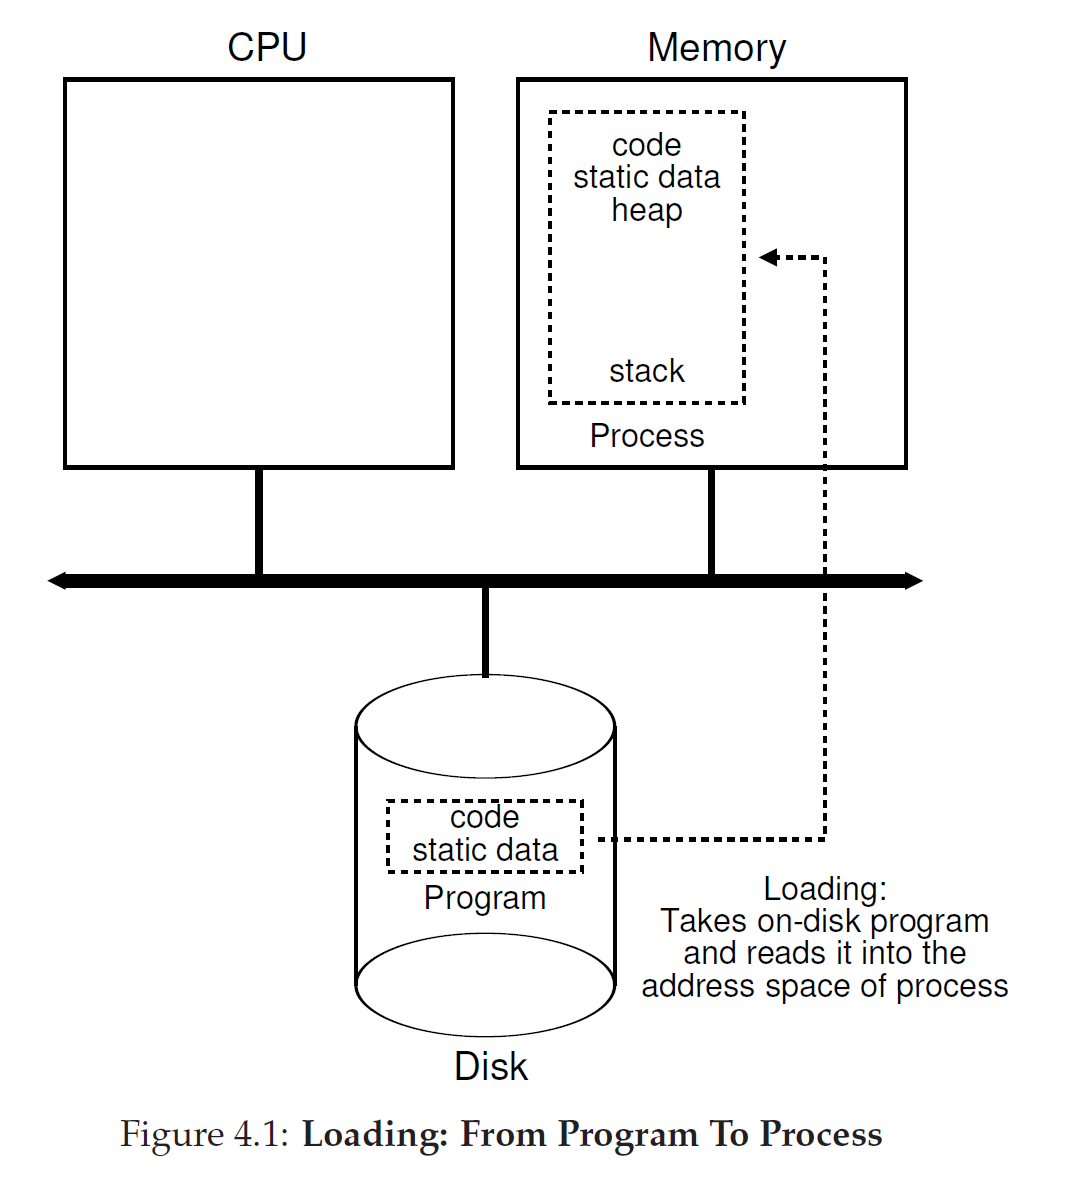
\includegraphics[width=13cm]{fig4.1.png}
    \caption{An image of a galaxy}
    \label{fig:galaxy}
\end{figure}

\textbf{\color{red}By jumping to the main() routine (through a specialized mechanism that we will discuss next chapter), the OS transfers control of the CPU to the newly-created process, and thus the program begins its execution.}

\subsubsection{Process States}
\begin{itemize}
    \item \textbf{Running: }In the running state, a process is running on a processor. This means it is executing instructions
    
    \item \textbf{Ready: }In the ready state, a process is ready to run but for some reason the OS has chosen not to run it at this given moment
    
    \item \textbf{Blocked: }In the blocked state, a process has performed some kind of operation that makes it not ready to run until some other event takes place. A common example: when a process initiates an I/O request to a disk, it becomes blocked and thus some other process can use the processor.
\end{itemize}

\begin{figure}[H]
    \centering
    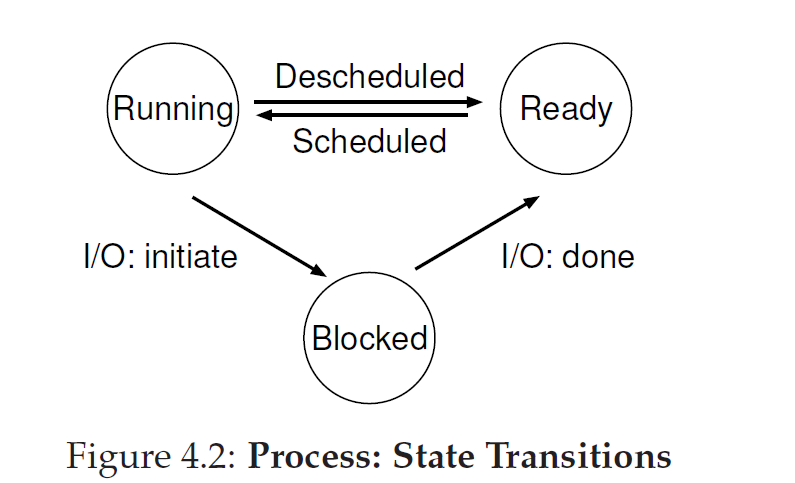
\includegraphics[width=13cm]  {fig4.2.png}
    \caption{An image of a galaxy}
    \label{fig:galaxy}
\end{figure}
a process can be moved between the ready and running states at the discretion of the OS. Being moved from ready to running means the process has been scheduled; being moved from running to ready means the process has been descheduled. Once a process has become blocked (e.g., by initiating an I/O operation), the OS will keep it as such until some event occurs (e.g., I/O completion); at that point, the process moves to the ready state again
(and potentially immediately to running again, if the OS so decides).
\begin{figure}[H]
    \centering
    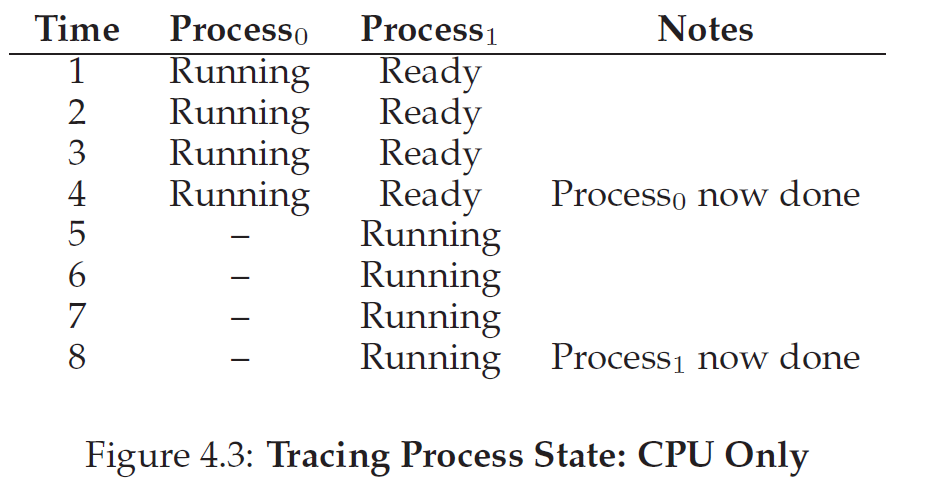
\includegraphics[width=13cm] {fig4.3.png}
    \caption{An image of a galaxy}
    \label{fig:galaxy}
\end{figure}

\begin{figure}[H]
    \centering
    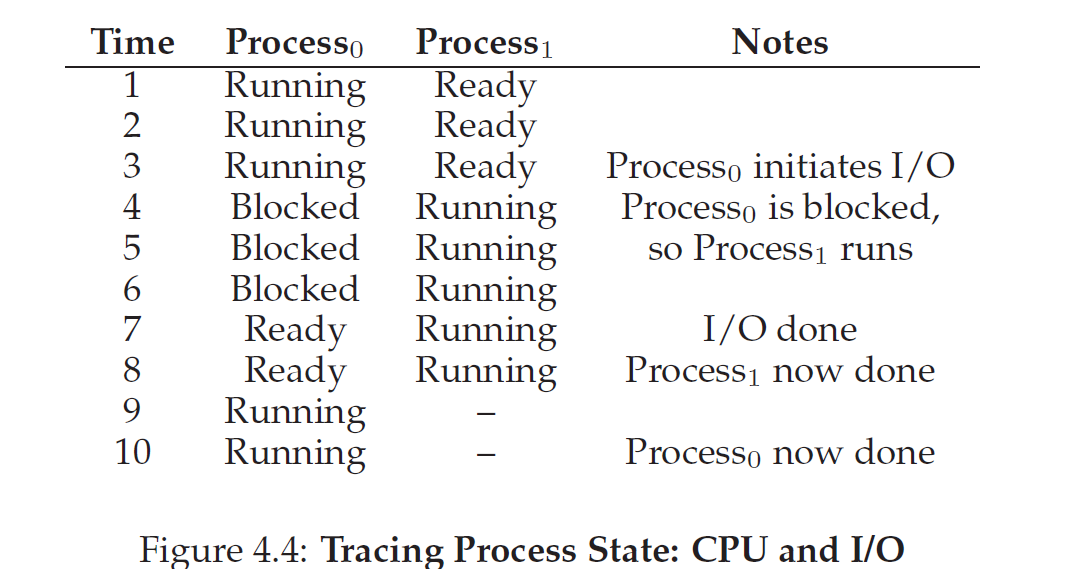
\includegraphics[width=13cm] {fig4.4.png}
    \caption{An image of a galaxy}
    \label{fig:galaxy}
\end{figure}


Process0 initiates an I/O and becomes blocked waiting for it to complete; processes become blocked, for example, when reading from a disk or waiting for a packet from a network. The OS recognizes
Process0 is not using the CPU and starts running Process1. While Process1 is running, the I/O completes, moving Process0 back to ready. Finally, Process1 finishes, and Process0 runs and then is done.


\subsubsection{Data Structures}
\begin{figure}[H]
    \centering
    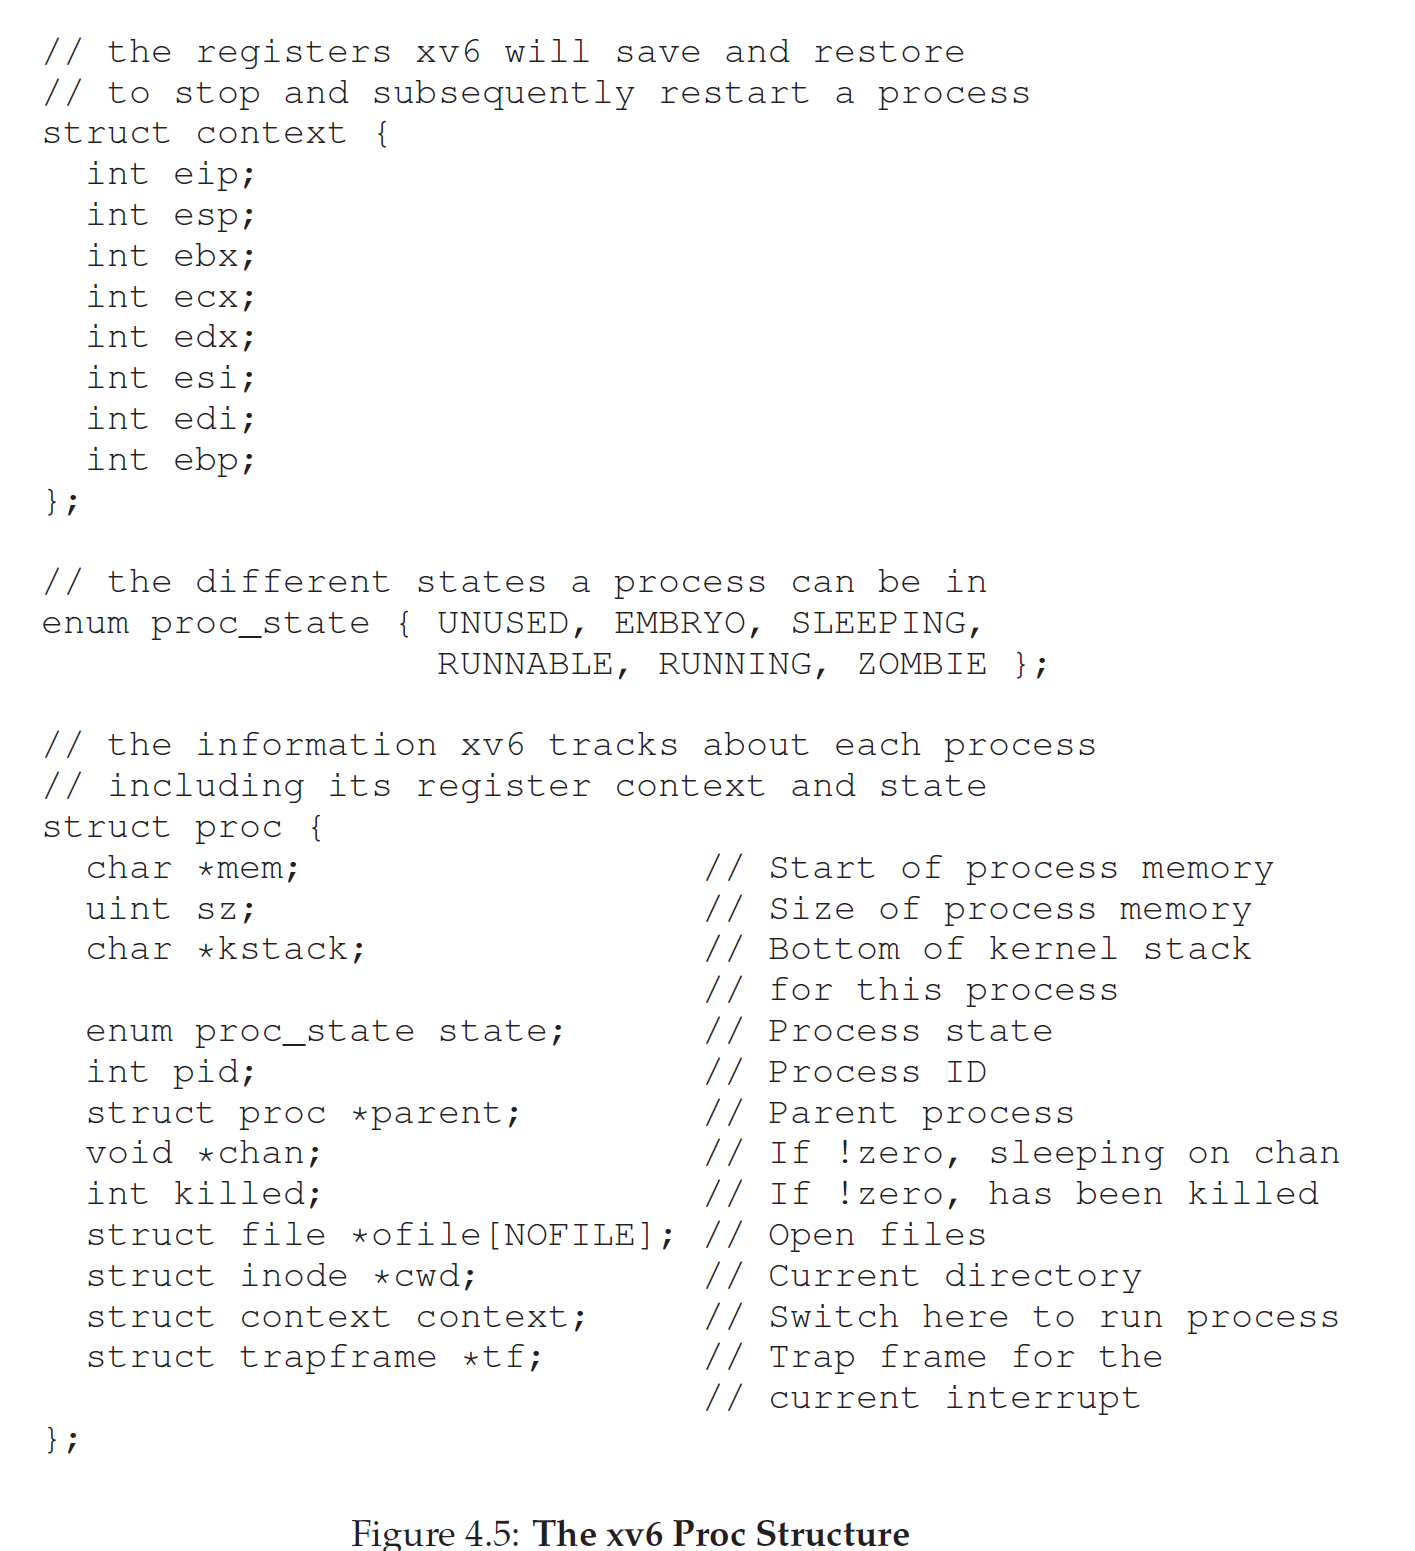
\includegraphics[width=13cm] {fig4.5.png}
    \caption{An image of a galaxy}
    \label{fig:galaxy}
\end{figure}
\textbf{process list} for all processes that are ready and some additional information
to track which process is currently running.
From the figure, you can see a couple of important pieces of information
the OS tracks about a process. The \textbf{register context} will hold, for a stopped process, the contents of its registers. When a process is stopped,
its registers will be saved to this memory location; by restoring these registers
(i.e., placing their values back into the actual physical registers), the
OS can resume running the process. We’ll learn more about this technique
known as a \textbf{context switch} in future chapters.
You can also see from the figure that there are some other states a process
can be in, beyond running, ready, and blocked. Sometimes a system
will have an \textbf{initial} state that the process is in when it is being created.
Also, a process could be placed in a \textbf{final} state where it has exited but has not yet been cleaned up (in UNIX-based systems, this is called the
\textbf{zombie state}). This final state can be useful as it allows other processes
(usually the \textbf{parent} that created the process) to examine the return code
of the process and see if the just-finished process executed successfully
(usually, programs return zero in UNIX-based systems when they have
accomplished a task successfully, and non-zero otherwise). When finished,
the parent will make one final call (e.g., wait()) to wait for the
completion of the child, and to also indicate to the OS that it can clean up
any relevant data structures that referred to the now-extinct process.

\pagebreak

\subsection{Process API (code)}
\pagebreak

\subsection{Machanism: Limited Direct Execution}
Achieve virtualization: by \textbf{time sharing}, run one process for a little while, then run another one, and so forth.\\
\textbf{Challenge: }Obtaining high performance while maintaining control is thus
one of the central challenges in building an operating system.
\begin{itemize}
    \item \textbf{performance: }how can we implement virtualization without adding excessive overhead to the system?
    \item \textbf{control: }how can we run processes efficiently while retaining control over the CPU?
\end{itemize}

\subsubsection{Basic Technique: Limited Direct Execution(LDE)}
\textbf{limited direct execution: }To make a program run as fast as one might expect

\begin{figure}[H]
    \centering
    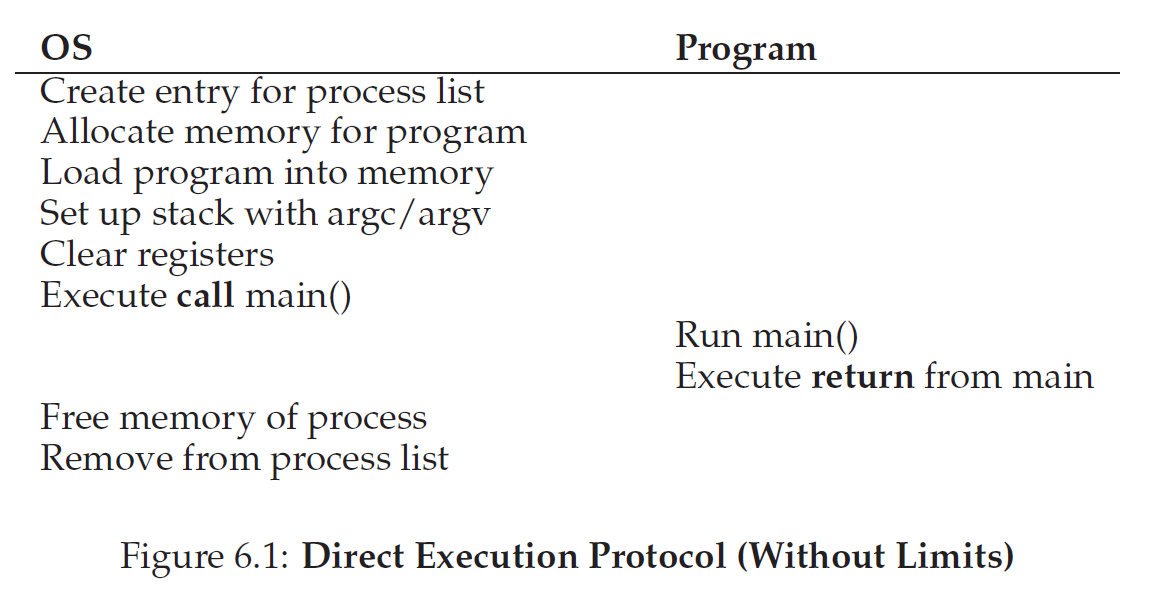
\includegraphics[width=13cm] {fig6.1.png}
    \caption{An image of a galaxy}
    \label{fig:galaxy}
\end{figure}

\textbf{Problems of unlimited direct execution:}
\begin{itemize}
    \item \textbf{control: }how can the OS make sure the program doesn’t do anything that we don’t want it to do, while still running it efficiently
    
    \item \textbf{implementing time sharing}
\end{itemize}


\subsubsection{Problem 1: Restricted Operations}
what if the process wishes to perform some kind of restricted operation, such as issuing an I/O request to a disk, or gaining access to more system resources such as CPU or memory?
\textbf{solution: }
\begin{itemize}
    \item \textbf{user mode: }code that runs in user mode is restricted in what it can do.
    
    \item \textbf{kernel mode: }In this mode, code that runs can do what it likes, including privileged operations such as issuing I/O requests and executing all types of restricted instructions. 
    
    \item \textbf{system call: }allow the kernel to carefully expose certain key pieces of functionality to user programs, such as accessing the file system, creating and destroying processes, communicating with other processes, and allocating more memory.
    \item \textbf{trap and return-from-trap}trap will jump into kernel and raise the privilege level to kernel mode; return-from-trap return into the calling user program while reducing the privilege level back to user mode.
    \item \textbf{trap table: }kernel control what code executes upon a trap
    
    \item \textbf{System-call number: }is usually assigned to each system call. The user code is thus responsible for placing the desired system-call number in a register or at a specified location on the stack; the OS, when handling the system call inside the trap handler, examines this number, ensures it is valid, and, if it is, executes the corresponding code. It's a protection
\end{itemize}
\begin{figure}[H]
    \centering
    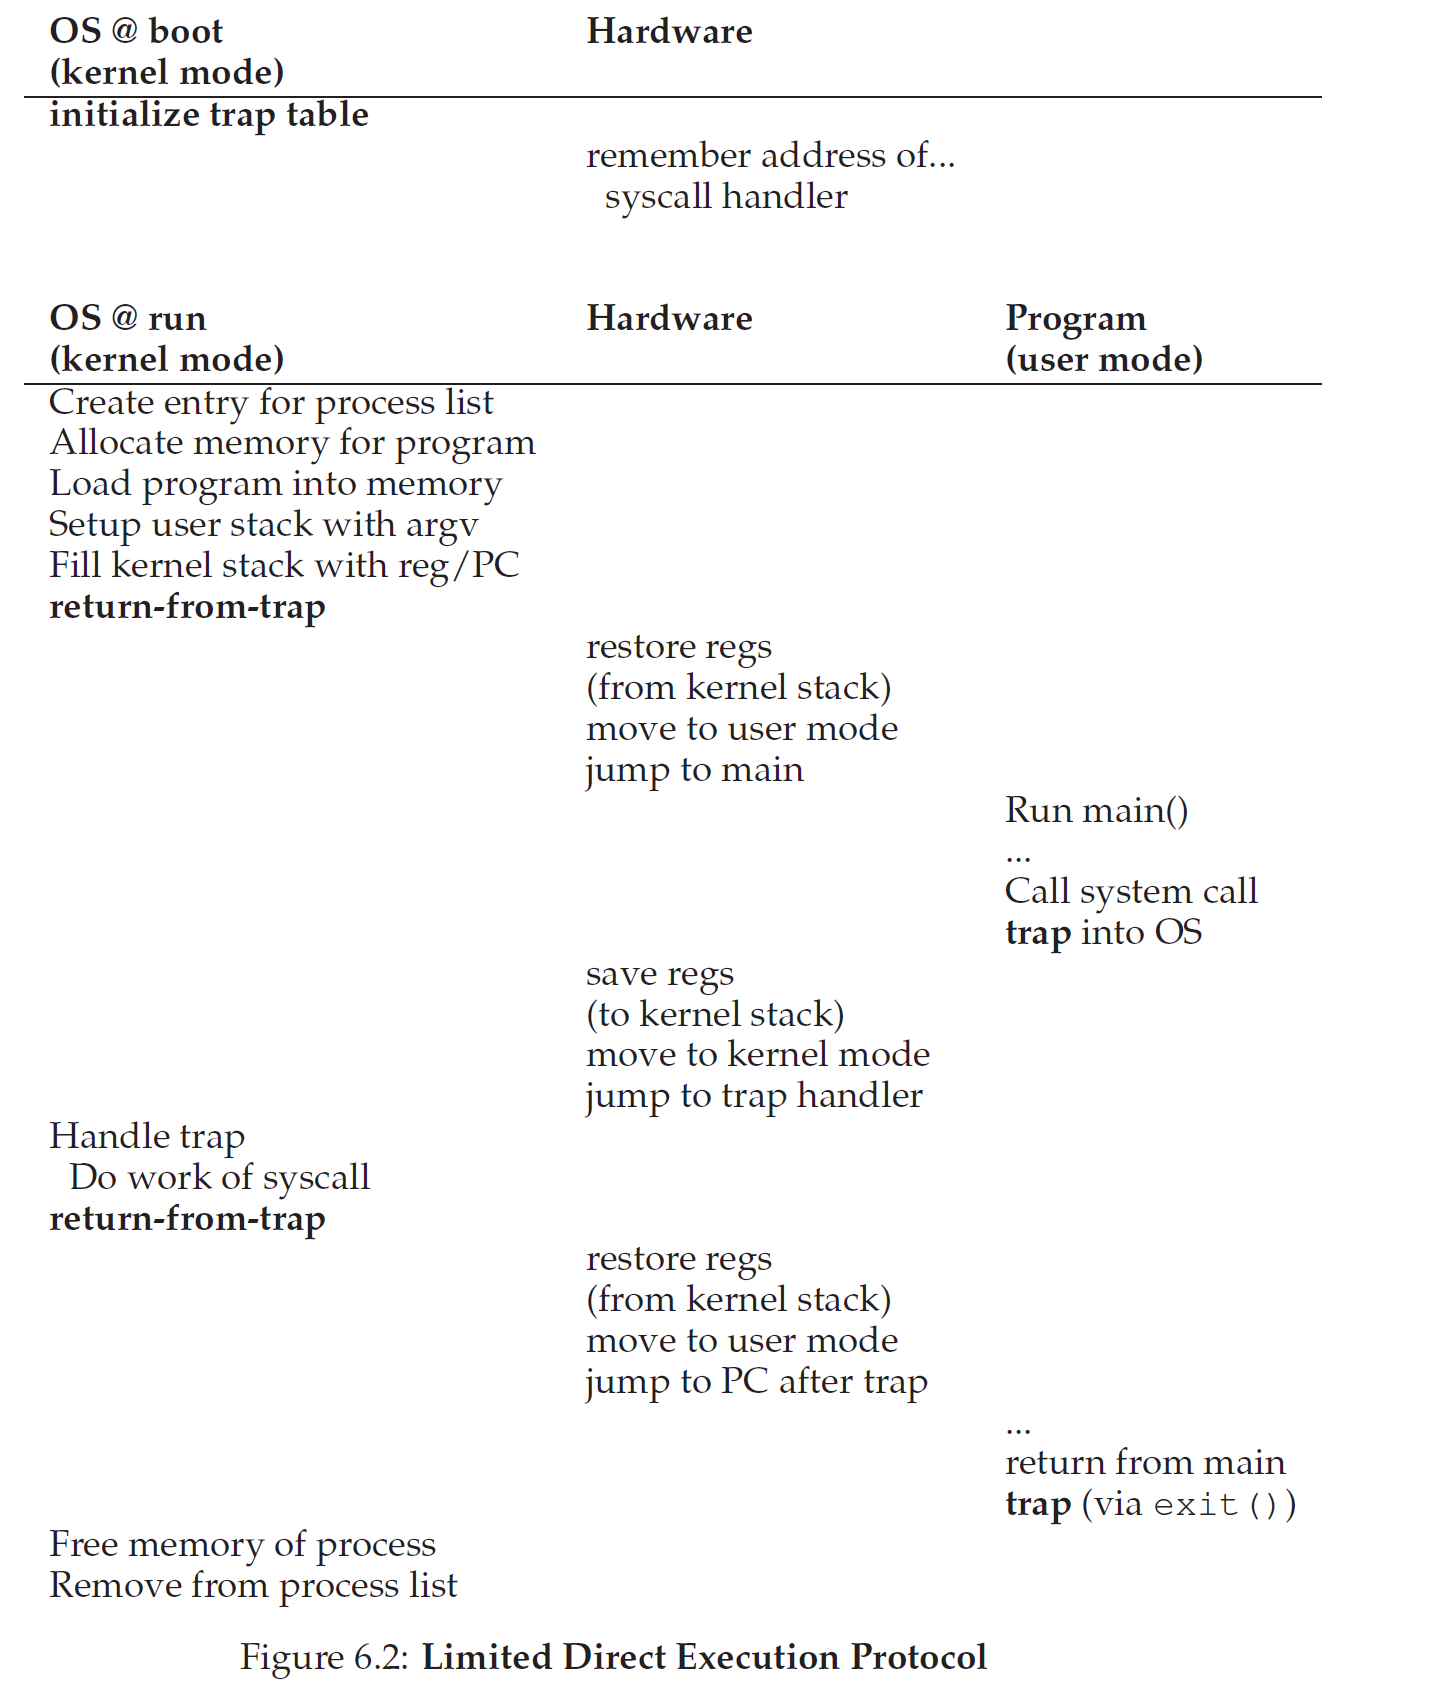
\includegraphics[width=13cm] {fig6.2.png}
    \caption{An image of a galaxy}
    \label{fig:galaxy}
\end{figure}
\textbf{2 phase in LDE}
\begin{itemize}
    \item \textbf{first phase(at boot time)} kernel initializes the trap table, and the CPU remembers its location for subsequent use. The kernel does so via a privileged instruction
    
    \item \textbf{second phase(when running a process): }
\end{itemize}

\subsubsection{problem 2: Switching Between Processes}
\textbf{\color{red}How can the operating system regain control of the CPU so that it can
switch between processes}

\begin{itemize}
    \item \textbf{A Cooperative Approach: Wait For System Calls}\\Thus, in a cooperative scheduling system, the OS regains control of the CPU by waiting for a system call or an illegal operation of some kind to take place. \textbf{\color{red}Problems: if a process (whether malicious, or just full of bugs) ends up in an infinite loop, and never makes a system call--reboot the machine.}
    
    \item \textbf{A Non-Cooperative Approach: The OS Takes Control--using timer interrupt}\\A timer device can be programmed to raise an interrupt every so many milliseconds; when the interrupt is raised, the currently running process is halted, and a pre-configured interrupt handler in the OS runs. At this point, the OS has regained control of the CPU, and thus can do what it pleases: stop the current process, and start a different one. At boot time, the OS must start the timer(
   privileged operation). The timer can also be turned off. \textbf{\color{red}Note that the hardware has some responsibility when an interrupt occurs, in particular to save enough of the state of the program that was running when the interrupt occurred such that a subsequent return-from trap instruction will be able to resume the running program correctly}
   
   \item \textbf{Saving and Restoring Context}\\
   OS make decision whether to continue running the currently-running process or switch to a different one.
   \begin{itemize}
       \item \textbf{switch: }execute a low-level piece of code: \textbf{\color{red} context switch}.all the OS has to do is save a few register values
for the currently-executing process (onto its kernel stack, for example)
and restore a few for the soon-to-be-executing process (from its kernel
stack). two types of register saves/restores: hardware and software
   \end{itemize}
\end{itemize}
\begin{figure}[H]
    \centering
    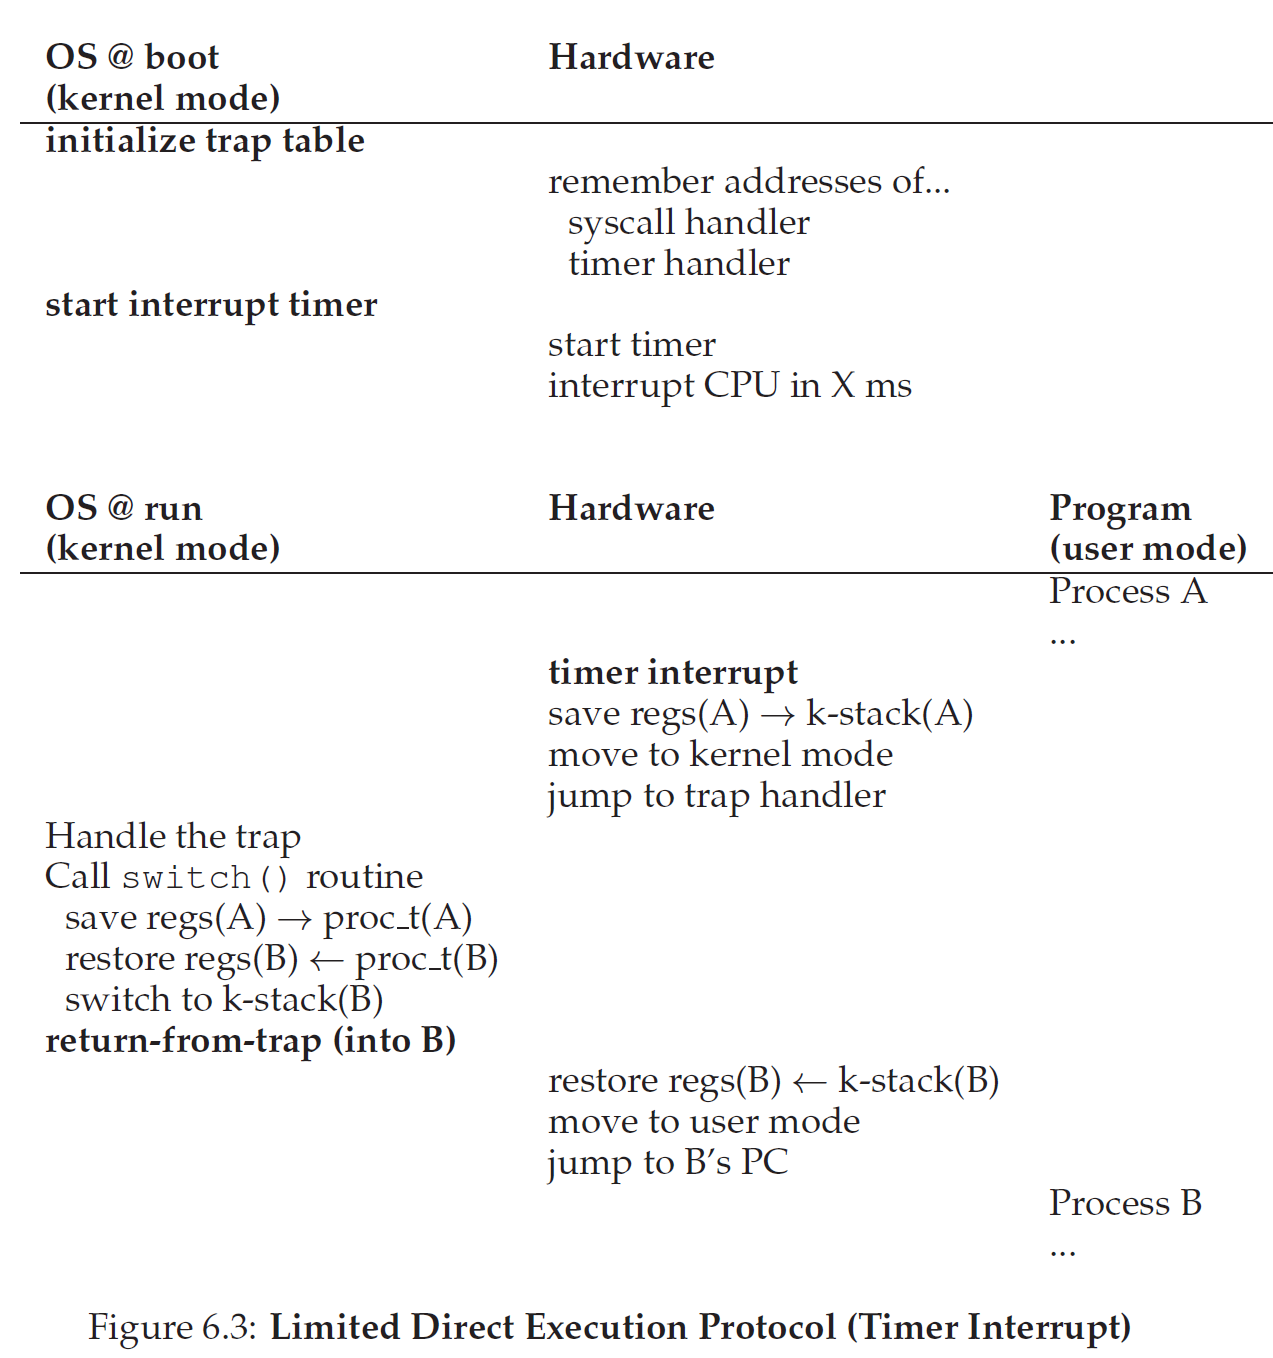
\includegraphics[width=13cm] {fig6.3.png}
    \caption{An image of a galaxy}
    \label{fig:galaxy}
\end{figure}

\subsubsection{Worried About Concurrency}
\begin{itemize}
    \item \textbf{disable interrupts during interrupt processing: }one interrupt is being handled, no other one will be delivered to the CPU.
    \item \textbf{locking schemes: }This enables multiple activities to be on-going within the kernel at the same time, particularly useful on multiprocessors.
\end{itemize}

\pagebreak
\pagebreak

\subsection{CPU Scheduling}

\subsubsection{Workload Assumptions}

\textbf{fully-operational scheduling discipline and assumptions}
\begin{itemize}
    \item Each job runs for the same amount of time.
    \item All jobs arrive at the same time
    \item Once started, each job runs to completion.
    \item All jobs only use the CPU (i.e., they perform no I/O)
    \item The run-time of each job is known.
\end{itemize}

\subsubsection{Scheduling Metrics}
{\color{red}Scheduling metric enables us to compare different scheduling polices}
{\color{red} Thus, if we knew job lengths, and that jobs only used the CPU, and our
only metric was turnaround time, STCF would be a great policy}
\begin{itemize}
    \item \textbf{turnaround time(Performance metric) }The turnaround time of a job is defined
as the time at which the job completes minus the time at which the job
arrived in the system.
$$T_{turnaround}=T_{completion}-T_{arrival}$$

\item \textbf{fairness: }optimize performance but at the cost of preventing a few jobs
from running, thus decreasing fairness.
\end{itemize}

\subsubsection{First In First Out Scheduling}
\textbf{Positive properties: }it is clearly simple and thus
easy to implement (assumed that each job runs for the same amount of time).\\
\textbf{disadvantage: convey effect }where
a number of relatively-short potential consumers of a resource get queued behind a heavyweight resource consumer.
\begin{figure}[H]
    \centering
    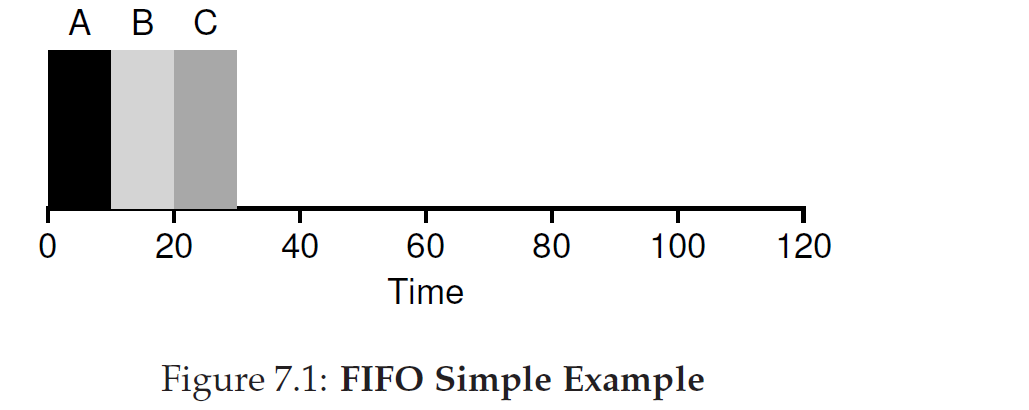
\includegraphics[width=13cm] {fig7.1.png}
    \caption{An image of a galaxy}
    \label{fig:galaxy}
\end{figure}
\begin{figure}[H]
    \centering
    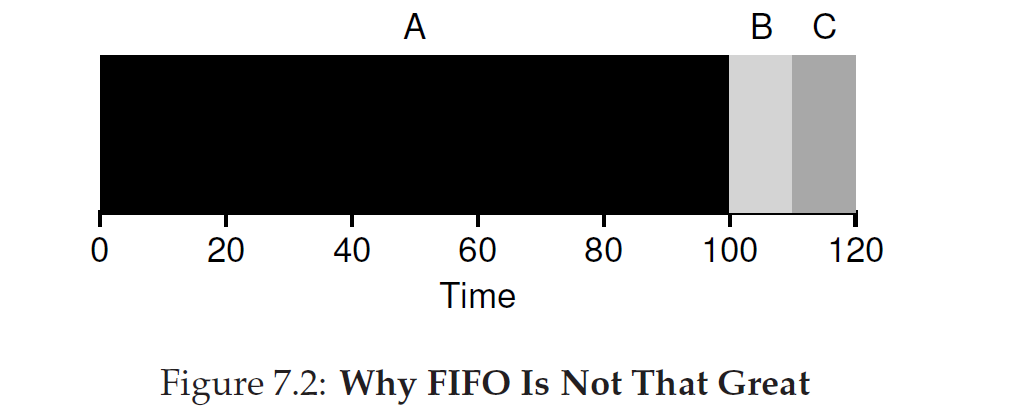
\includegraphics[width=13cm] {fig7.2.png}
    \caption{An image of a galaxy}
    \label{fig:galaxy}
\end{figure}
\subsubsection{Shortest Job First(SJF)}
\textbf{\color{red} Non-preemptive scheduler}
{\color{red}it runs the
shortest job first, then the next shortest, and so on. It assumes that all jobs arriving at the same time.}
\textbf{problems: convoy effect} short jobs coming later still have to wait for the first coming long task to finish
\begin{figure}[H]
    \centering
    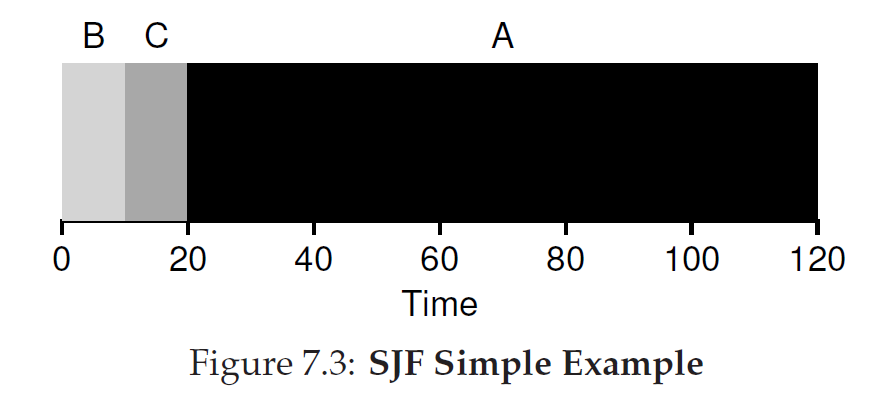
\includegraphics[width=13cm] {fig7.3.png}
    \caption{An image of a galaxy}
    \label{fig:galaxy}
\end{figure}
\begin{figure}[H]
    \centering
    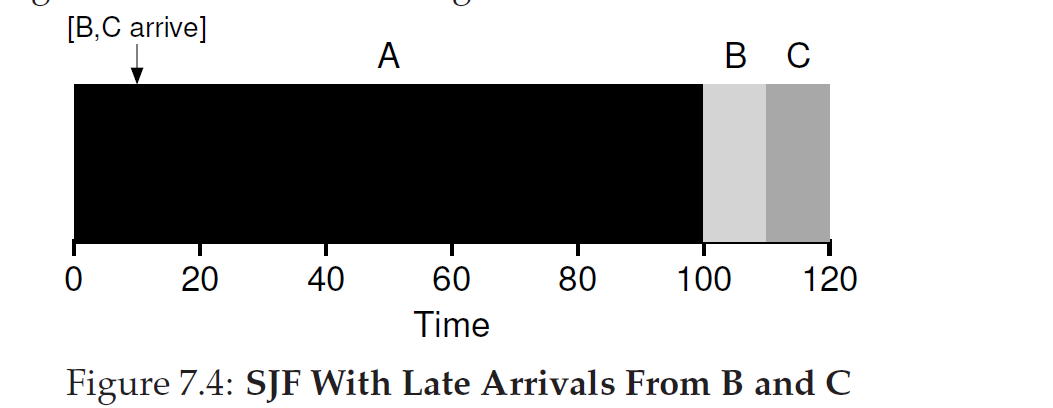
\includegraphics[width=13cm] {fig7.4.png}
    \caption{An image of a galaxy}
    \label{fig:galaxy}
\end{figure}

\subsubsection{Shortest Time-to-Completion First (STCF)}
\textbf{relax the assumption: jobs must
run to completion}.\\
scheduler can preempt job A and decide to run another job and continuing A later.
\textbf{\color{red} Preemptive Shortest Job First scheduler: }Any time a new
job enters the system, the STCF scheduler determines which of the remaining
jobs (including the new job) has the least time left, and schedules
that one.
\begin{figure}[H]
    \centering
    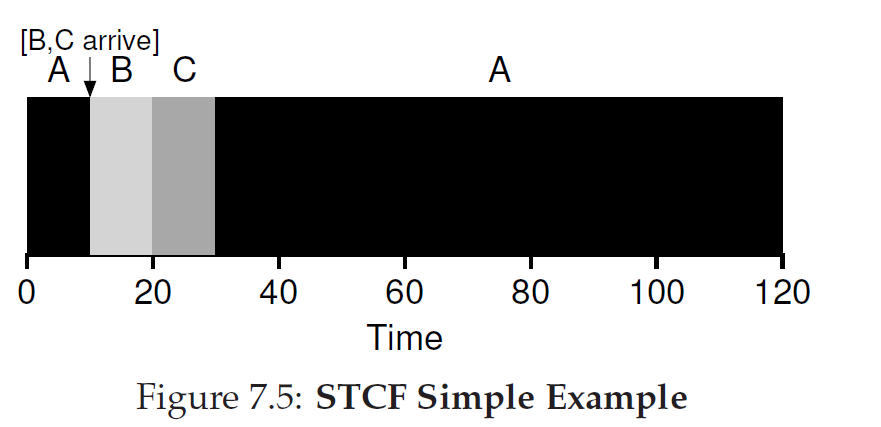
\includegraphics[width=13cm] {fig7.5.png}
    \caption{An image of a galaxy}
    \label{fig:galaxy}
\end{figure}

\subsubsection{A New Metric: Response Time}
$$T_{response}=T_{firstscheduled}-T_{arrival}$$
{\color{red}STCF and related disciplines are not particularly
good for response time.}If three jobs arrive at the same time,
for example, the third job has to wait for the previous two jobs to run in their entirety before being scheduled just once. While great for turnaround time, this approach is quite bad for response time and interactivity



\subsubsection{Round Robin--sensitive to response time}
\begin{figure}[H]
    \centering
    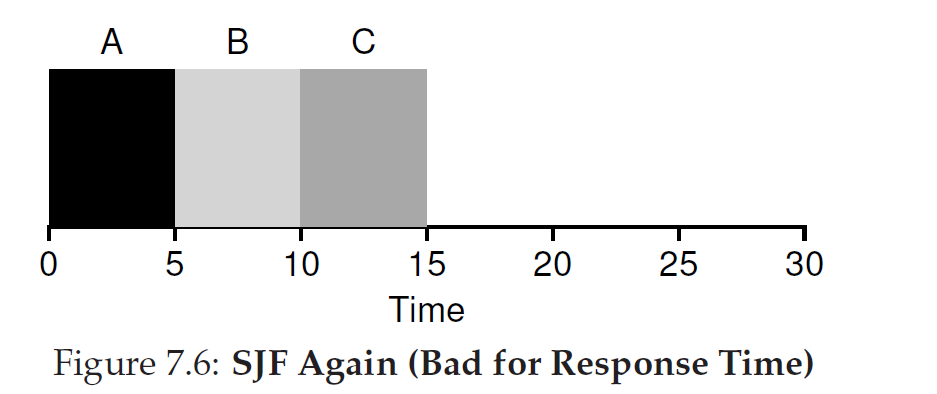
\includegraphics[width=13cm] {fig7.6.png}
    \caption{An image of a galaxy}
    \label{fig:galaxy}
\end{figure}
\begin{figure}[H]
    \centering
    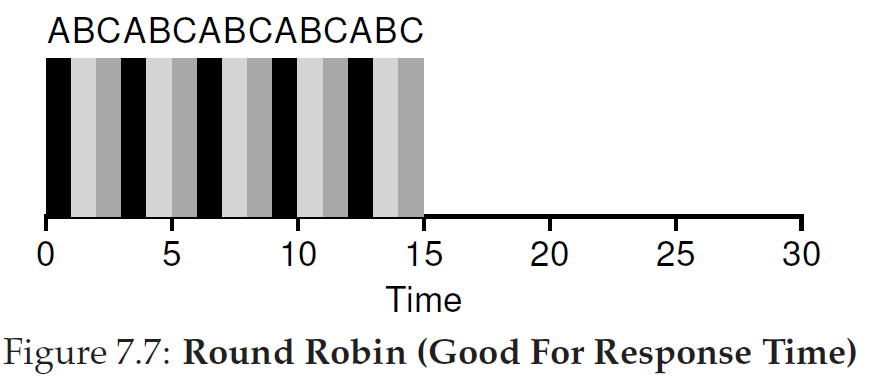
\includegraphics[width=13cm] {fig7.7.png}
    \caption{An image of a galaxy}
    \label{fig:galaxy}
\end{figure}
{\color{red}Also called time-slicing. Instead of running jobs to completion, RR runs a job for a
time slice (sometimes called a scheduling quantum) and then switches to the next job in the run queue. It repeatedly does so until the jobs are
finished.} Note that
the length of a time slice must be a multiple of the timer-interrupt period;
thus if the timer interrupts every 10 milliseconds, the time slice could be
10, 20, or any other multiple of 10 ms.

{\color{red} Note that
the length of a time slice must be a multiple of the timer-interrupt period;
thus if the timer interrupts every 10 milliseconds, the time slice could be
10, 20, or any other multiple of 10 ms. But the
cost of context switching will dominate overall performance.}

\textbf{AMORTIZATION CAN REDUCE COSTS: }deciding
on the length of the time slice presents a trade-off to a system designer,
making it long enough to amortize the cost of switching without
making it so long that the system is no longer responsive.

{\color{red}RR, with a reasonable time slice, is thus an excellent scheduler if response
time is our only metric}

{\color{red} SJF, STCF optimizes turnaround time, but is bad for response time. RR optimizes response time but is bad for turnaround}

\subsubsection{Incorporating I/O}
A scheduler clearly has a decision to make when a job initiates an I/O
request, because the currently-running job won’t be using the CPU during
the I/O;The scheduler also has to make a decision when the I/O completes.
When that occurs, an interrupt is raised, and the OS runs and moves
the process that issued the I/O from blocked back to the ready state.
While those interactive jobs are performing
I/O, other CPU-intensive jobs run, thus better utilizing the processor.

\begin{figure}[H]
    \centering
    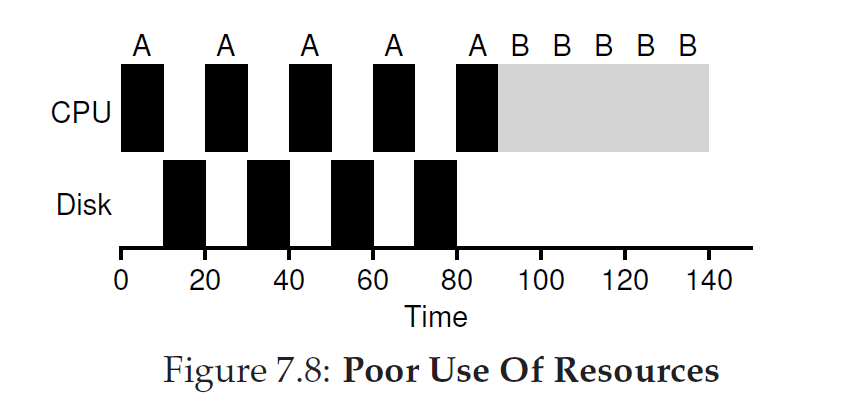
\includegraphics[width=13cm] {fig7.8.png}
    \caption{An image of a galaxy}
    \label{fig:galaxy}
\end{figure}
\begin{figure}[H]
    \centering
    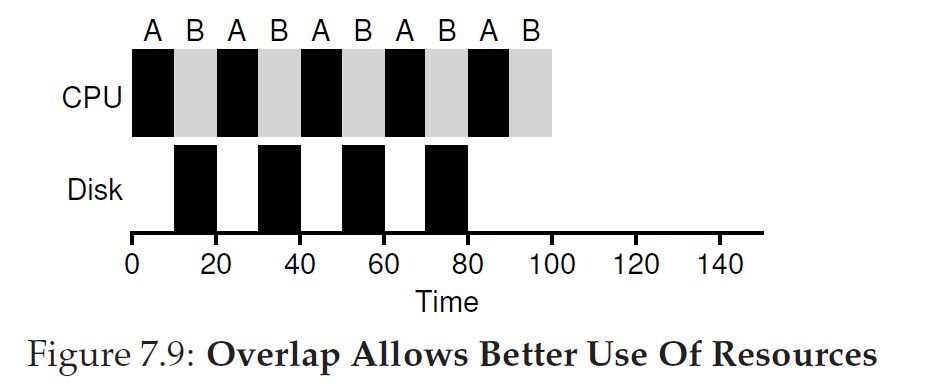
\includegraphics[width=13cm] {fig7.9.png}
    \caption{An image of a galaxy}
    \label{fig:galaxy}
\end{figure}
\pagebreak

\subsection{Multi-level Feedback Queue}
\textbf{\color{red} 1.optimize turnaround time by running shorter jobs first. But OS doesn’t generally know how long a job will run for, exactly the knowledge that algorithms like SJF (or STCF) require\\ 2.Minimize response time for interactive jobs}

\subsubsection{MLFQ: Basic Rules}
\subsection{Lottery Scheduling(code)}
\subsection{Multi-CPU Scheduling}
\subsection{Summary}
\end{document}
